%%%NOTE: for help with latex symbols look here http://mirror.unl.edu/ctan/info/symbols/comprehensive/symbols-a4.pdf.
\documentclass[12pt]{article}
\usepackage{color}
\usepackage{cite}
\usepackage{geometry}                % See geometry.pdf to learn the layout options. There are lots.
%\usepackage{pdflscape}        %single page landscape
                                %mode \begin{landscape} \end{landscape}
\geometry{letterpaper}                   % ... or a4paper or a5paper or ... 
%\usepackage[parfill]{parskip}    % Activate to begin paragraphs with an empty line rather than an indent
\usepackage{multicol} % \begin{multicols}{number of columns} \end{multicols}
% \usepackage{lineno} %add lines numbers 
\usepackage{graphicx}
\usepackage{amssymb}
\usepackage{Sweave}
\newcommand{\etal}{\textit{et al.}}
\usepackage{hyperref}  %\hyperref[label_name]{''link text''}
                       %\hyperlink{label}{anchor caption}
                       %\hypertarget{label}{link caption}
\linespread{1.5}

\title{Unstable States: Community dynamics in a chaotic world}
\author{M.K. Lau}
%\date{}                                           % Activate to display a given date or no date

\begin{document}
\maketitle
%\linenumbers %%add line numbers

%\setcounter{tocdepth}{3}  %%activate to number sections
%\tableofcontents

%\thispagestyle{empty}
%\setcounter{page}{0}
%\setcounter{secnumdepth}{-1}  %activate to start numbering from one
%on the second page

\section{8 Jul 2014}


Eigenvalues indicate system dynamics.

A system is stable if it eventually returns to a fixed point after a
disturbance.

A system is unstable if it is not stable.

For imaginary (complex) eigenvalues:

\begin{itemize}
\item Negative Real Part - Stable. Damping is a requirement of stability. 
\item Positive Real Part - Unstable. Increasing amplitude is unstable.
\item Zero Real Part - Unstable. Oscillators are unstable, as they
  will not go back to a steady state post-disturbance
\item The complex part will not affect the stability. 
\end{itemize}

Real eigenvalues:
\begin{itemize}
\item Zero eigenvalues: unstable
\item All Positive: unstable
\item All Negative: unstable
\item Both positive and negative: unstable, saddle.
\item Repeated: needs further analysis. For the special case of two
  eigenvalues, both positive = unstable, both negative = stable.
\end{itemize}

Check out this figure:

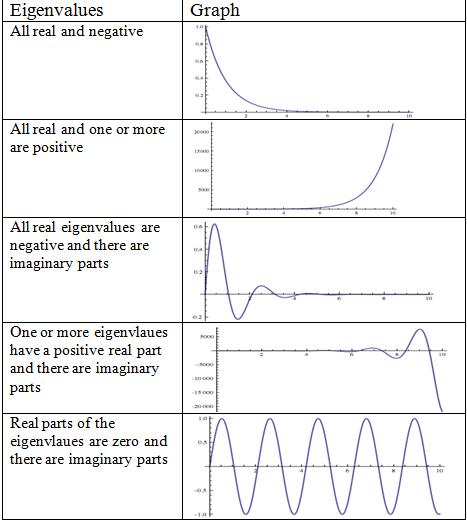
\includegraphics[]{../docs/Eigenvalue_graphs.jpg}


\begin{Schunk}
\begin{Sinput}
>   source('../src/sens2_ews.R')
> library(ecodist)
> fps <- read.csv('~/Dropbox/Tipping Point MS/Model sensitivity analysis and second paper/data/parameters.csv') 
> x <- read.csv('~/Dropbox/Tipping Point MS/Model sensitivity analysis and second paper/data/hundred_min_average.csv')
> x <- x[,-1]
> x <- x[1:12500,]
> x[x<0] <- 0
> x <- t(x)
> 
> ##Obtain equations
> 
> 
\end{Sinput}
\end{Schunk}

\section{3 Jul 2014}

\textit{Foundations of Resilience Thinking}

\begin{itemize}
\item Resilience = size and steepness of attractor basins
\item Distinguishes between: near equilibrium behavior and long term persistence
\item Panarchy = Processes operating at different scales permit organization
\end{itemize}

\textit{How does NMDS treat mutual information?}

\begin{Schunk}
\begin{Sinput}
>   source('../src/sens2_ews.R')
> library(ecodist)
> fps <- read.csv('~/Dropbox/Tipping Point MS/Model sensitivity analysis and second paper/data/parameters.csv') 
> x <- read.csv('~/Dropbox/Tipping Point MS/Model sensitivity analysis and second paper/data/hundred_min_average.csv')
> x <- x[,-1]
> x <- x[1:12500,]
> x[x<0] <- 0
> x <- t(x)
> ###kernel density information
> d1 <- density(x[1,])
> d2 <- density(x[2,])
> plot(density(x[1,])$x,density(x[3,])$x)
> points(-2:12,-2:12)
> 
> ###
> 
> 
> 
\end{Sinput}
\end{Schunk}


\section{2 Jul 2014}

Mutual Information for Time Series

This is an attempt to implement methods from Moniz et al. (2007)
Application of Information Theory Methods to Food Web Reconstruction

\begin{Schunk}
\begin{Sinput}
>   source('../src/sens2_ews.R')
> library(entropy)
> library(vegan)
> library(ecodist)
> fps <- read.csv('~/Dropbox/Tipping Point MS/Model sensitivity analysis and second paper/data/parameters.csv') 
> x <- read.csv('~/Dropbox/Tipping Point MS/Model sensitivity analysis and second paper/data/hundred_min_average.csv')
> x <- x[,-1]
> x <- x[1:12500,]
> x[x<0] <- 0
> x <- t(x)
> ###
> ## mid.m <- array(0,dim=c(nrow(x),nrow(x)))
> ## for (i in 1:nrow(x)){
> ##   for (j in 1:nrow(x)){
> ##     mid.m[i,j] <- mi.Dirichlet(x[c(i,j),],0.5)
> ##   }
> ## }
> mid.m <- dget(file='../data/midm.rda')
> mid.m <- round(mid.m,7)
> pca <- princomp(as.dist(mid.m))
> nms <- nmds.min(nmds(as.dist(mid.m),2,2))
> plot(nms)
> plot(envfit(env=fps,ord=nms))
> envfit(env=fps,ord=nms)
> 
\end{Sinput}
\end{Schunk}

\begin{Schunk}
\begin{Sinput}
>   library(entropy)
> y2d <- rbind( sample(1:100,100), sample(1:100,100) )
> y2d. = rbind( sample(1:100,100), sample(1:100,100) )
> test <- test. <- 0
> a <- seq(0,1,by=0.01)
> for (i in 1:length(a)){test[i] <- mi.Dirichlet(y2d,a=a[i])}
> for (i in 1:length(a)){test.[i] <- mi.Dirichlet(y2d.,a=a[i])}
> plot(test.~test);abline(lm(range(test.)~range(test)))
> 
\end{Sinput}
\end{Schunk}



\section{1 Jul 2014}

Reading Beltrami:

\begin{Schunk}
\begin{Sinput}
> ##For N. = rN
> ##N(t) = N(0)e^rt
> 
> N0 <- seq(0,100,by=0.1)
> t <- 0:100
> Nt <- sapply(N0, function(N0,t,r) N0*exp(r*t),t=t,r=2)
> plot(Nt[,1]~t,xlim=range(t),ylim=range(Nt),type='l',)
> for (i in 2:ncol(Nt)){lines(Nt[,i]~t)}
> plot(apply(Nt,2,max)~N0,type='l')
> plot(Nt[,ncol(Nt)]~t,xlim=range(t),ylim=range(Nt),type='l',)
> 
\end{Sinput}
\end{Schunk}

\section{30 Jun 2014}



\begin{Schunk}
\begin{Sinput}
>   library('nimble')
> 
\end{Sinput}
\end{Schunk}

\section{27 Jun 2014}
Alternative state detection?
Should we be looking for break points?

\begin{Schunk}
\begin{Sinput}
> source('../src/sens2_ews.R')
>   fps <- read.csv('~/Dropbox/Tipping Point MS/Model sensitivity analysis and second paper/data/parameters.csv') 
> x <- read.csv('~/Dropbox/Tipping Point MS/Model sensitivity analysis and second paper/data/hundred_min_average.csv')
> x <- x[,-1]
> x <- x[1:12500,]
> x[x<0] <- 0
> ###
> my.col <- rainbow(nlevels(factor(fps$Prey)))[as.numeric(factor(fps$Prey))]
> ###
> cx <- x[,5]
> cx[cx<=0.03] <- 0
> plot(cx)
> abline(v=find.days(cx)$start)
> abline(v=find.days(cx)$end)
> days <- find.days(cx)
> x.days <- apply(x,2,function(x,d) x[d],d=sort(unlist(days)))
> x.cor <- list()
> for (k in 1:ncol(x)){
+   out <- 0
+   for (i in 1:(length(days)-1)){
+     d1 <- days[[i]]
+     d2 <- days[[(i+1)]]
+     xt <- x[d1[1:min(c(length(d1),length(d2)))],k]
+     xt1 <- x[d2[1:min(c(length(d1),length(d2)))],k]
+     out[i] <- cor(xt,xt1,method='k')
+   }
+   x.cor[[k]] <- out
+ }
> plot(x.cor[[1]],type='l',ylim=c(-0.5,1),xlab='Day',col=my.col[[1]])
> for (i in 1:length(x.cor)){lines(x.cor[[i]],col=my.col[[i]])}
> ###
> par(mfcol=c(2,1))
> i <- 1
> plot(density(x[,i]),main='',xlab=expression(O[2]),
+      xlim=range(x)+c(-1,1),ylim=c(0,1),col=my.col[i])
> for (i in 2:ncol(x)){
+   x.dens <- density(x[,i])
+   x.dens$y <- x.dens$y/max(x.dens$y)
+   x.dens$y <- x.dens$y+runif(1,-0.025,0.025)
+   lines(x.dens,col=my.col[i])
+ }
> legend('topright',legend=levels(factor(fps$Prey)),lty=1,col=rainbow(nlevels(factor(fps$Prey))),title='Prey')
> ##
> my.col <- rainbow(nlevels(factor(fps$Prey)))[as.numeric(factor(fps$Prey))]
> i <- 1
> plot(1:nrow(x)~x[,i],col=my.col[i],xlab=expression(O[2]),ylab='time',type='l')
> for (i in 2:ncol(x)){
+   lines(1:nrow(x)~x[,i],col=my.col[i],xlab=expression(O[2]),ylab='time',type='l')
+ }
> 
> ###Calculate the correlation between days
> 
> 
\end{Sinput}
\end{Schunk}



\section{26 Jun 2014}
- Sub-sample
- Standardize, detrend and decycle
- Euclidean distance
- Plot of eigen values
- PC plot
- overlay vectors

\begin{Schunk}
\begin{Sinput}
> library(vegan)
> library(ecodist)
> source('../src/sens2_ews.R')
>   fps <- read.csv('~/Dropbox/Tipping Point MS/Model sensitivity analysis and second paper/data/parameters.csv') 
> x <- read.csv('~/Dropbox/Tipping Point MS/Model sensitivity analysis and second paper/data/hundred_min_average.csv')
> x <- x[,-1]
> x <- x[1:12500,]
> x[x<0] <- 0
> ###standardize, detrend and decycle
> sdd.x <- list()
> index <- apply(fps,1,function(x) paste(x[3:6],collapse=' '))
> cn <- (1:nrow(fps))[fps$Prey==0&index==paste(fps[1,3:6],collapse=' ')]
> for (i in 1:ncol(x)){
+   if (all(x[,i]==0)){sdd.x[[i]] <- NA}else{
+     cn <- (1:nrow(fps))[fps$Prey==0&index==paste(fps[i,3:6],collapse=' ')]  
+     sdd.x[[i]] <- sddSens(x[,i],x[,cn],eval=6250)
+   }
+ }
> sdd.x <- do.call(cbind,sdd.x)
> sdd.x[is.na(sdd.x)] <- 0
> ###ordinate
> sdd.d <- dist(t(sdd.x))
> hist(sdd.d)
> plot(hclust(sdd.d))
> ##
> par(mfrow=c(1,3))
> plot(sdd.x[,1],xlab='time',ylab=expression(O[2]),ylim=c(-1,1),pch=19,cex=0.05)
> for (i in 1:ncol(sdd.x)){points(sdd.x[,i],pch=19,cex=0.05)}
> sdd.ord <- princomp(sdd.d)
> names(sdd.ord)
> plot(sdd.ord$sdev/sum(sdd.ord$sdev))
> abline(h=0.05,lty=2)
> plot(sdd.ord$scores[,1:2])
> plot(envfit(ord=sdd.ord$scores[,1:2],env=fps))
> ###
> envfit(ord=sdd.ord$scores[,1:2],env=fps)
> envfit(ord=sdd.ord$scores[,2:3],env=fps)
> envfit(ord=sdd.ord$scores[,1:3],env=fps)
> pairs(fps)
> pairs(sdd.ord$scores[,1:3],pch=19,cex=1)
> par(mfrow=c(3,3))
> for (i in 1:3){
+   for (j in 1:3){
+     if (i==j){
+       plot(c(-1,1),c(-1,1),pch='',xlab='',ylab='',xaxt='n',yaxt='n')
+       text(c(0,0),c(0,0),labels=i,cex=5)
+     }else{
+       plot(sdd.ord$scores[,j:i],pch=19,cex=0.75)
+       plot(envfit(ord=sdd.ord$scores[,j:i],env=fps))
+   }
+   }
+ }
> library(rgl)
> plot3d(sdd.ord$scores[,1:3],type='s',col=rainbow(nlevels(factor((fps$Prey))))[as.numeric(factor((fps$Prey)))])
> plot3d(sdd.ord$scores[,1:3],type='s',col=rainbow(nlevels(factor((fps$b))))[as.numeric(factor((fps$b)))])
> plot3d(sdd.ord$scores[,1:3],type='s',col=rainbow(nlevels(factor((fps$a))))[as.numeric(factor((fps$a)))])
> plot3d(sdd.ord$scores[,1:3],type='s',col=rainbow(nlevels(factor((fps$K))))[as.numeric(factor((fps$K)))])
> plot3d(sdd.ord$scores[,1:3],type='s',col=rainbow(nlevels(factor((fps$d))))[as.numeric(factor((fps$d)))])
> 
\end{Sinput}
\end{Schunk}

\section{20 Jun 2014}

Plot tests (ordination and smoothed-detrended-decycled) are up on
github.

EWS for simulations:

- Write a script that will record the early warning signals for all
180 simulations.

\begin{Schunk}
\begin{Sinput}
> source('../src/sens2_ews.R')
>   fps <- read.csv('~/Dropbox/Tipping Point MS/Model sensitivity analysis and second paper/data/parameters.csv') 
> x <- read.csv('~/Dropbox/Tipping Point MS/Model sensitivity analysis and second paper/data/hundred_min_average.csv')
> x <- x[,-1]
> #x <- x[1000:5400,]
> x[x<0] <- 0
> ###Isolate controls
> my.col <- rainbow(nlevels(factor(fps$Prey)))[as.numeric(factor(fps$Prey))]
> sdd.x <- list()
> index <- apply(fps,1,function(x) paste(x[3:6],collapse=' '))
> cn <- (1:nrow(fps))[fps$Prey==0&index==paste(fps[1,3:6],collapse=' ')]
> plot(sdd.x[[1]] <- sddSens(x[,1],x[,cn]),ylim=c(-1,1),pch=19,
+      cex=0.25,ylab=expression(O[2]),xlab='t',col=my.col[1])
> for (i in 1:ncol(x)){
+   if (all(x[,i]==0)){sdd.x[[i]] <- NA}else{
+     cn <- (1:nrow(fps))[fps$Prey==0&index==paste(fps[i,3:6],collapse=' ')]  
+     points(sdd.x[[i]] <- sddSens(x[,i],x[,cn]),pch=19,cex=0.25,col=my.col[i])
+   }
+ }
> legend('topright',legend=unique(fps$Prey),col=rainbow(nlevels(factor(fps$Prey))),pch=19,title=expression(w[0]))
> ###
> par(mfrow=c(1,2))
> plot(x[,1])
> plot(sdd.x[[1]])
> ###
> my.col <- rainbow(nlevels(factor(fps$b)))[as.numeric(factor(fps$b))]
> sdd.x <- list()
> index <- apply(fps,1,function(x) paste(x[3:6],collapse=' '))
> cn <- (1:nrow(fps))[fps$Prey==0&index==paste(fps[1,3:6],collapse=' ')]
> plot(sdd.x[[1]] <- sddSens(x[,1],x[,cn]),ylim=c(-1,1),pch=19,
+      cex=0.25,ylab=expression(O[2]),xlab='t',col=my.col[1])
> for (i in 1:ncol(x)){
+   if (all(x[,i]==0)){sdd.x[[i]] <- NA}else{
+     cn <- (1:nrow(fps))[fps$Prey==0&index==paste(fps[i,3:6],collapse=' ')]  
+     points(sdd.x[[i]] <- sddSens(x[,i],x[,cn]),pch=19,cex=0.25,col=my.col[i])
+   }
+ }
> legend('topright',legend=levels(factor(fps$b)),col=rainbow(nlevels(factor(fps$b))),pch=19,title='b')
> library(strucchange)
> 
> 
\end{Sinput}
\end{Schunk}

Look at the temporal correlation structure among simulations:

\begin{Schunk}
\begin{Sinput}
> ##Using the 100 min averages
> ##Runs are in columns
>   fps <- read.csv('~/Dropbox/Tipping Point MS/Model sensitivity analysis and second paper/data/parameters.csv') 
> x <- read.csv('~/Dropbox/Tipping Point MS/Model sensitivity analysis and second paper/data/hundred_min_average.csv')
> x <- x[,-1]
> plot(x[,1],xlab='t',ylab=expression(O[2]),ylim=c(0,max(x)),type='l',lwd=0.5,col=rainbow(ncol(x))[1])
> for (i in 2:ncol(x)){
+   lines(1:nrow(x),x[,i],lwd=0.5,col=rainbow(ncol(x))[i])
+ }
> abline(v=c(1000,5400))
> x <- x[1000:5400,]
> x[x<0] <- 0
> d.x <- dist(t(x))
> library(vegan)
> library(ecodist)
> eig.x <- eigen(d.x)
> biplot(princomp(d.x))
> vd.x <- vegdist(t(rbind(x,rep(1,ncol(x)))))
> nmds.x <- nmds(vd.x,2,2)
> envf.x <- envfit(env=fps,ord=nmds.min(nmds.x))
> plot(apply(nmds.min(nmds.x),2,jitter,factor=50),col=rainbow(ncol(x)))
> plot(envf.x)
> envf.x
> 
\end{Sinput}
\end{Schunk}

\section{19 Jun 2014}

Generate plots for the tipping_points2

\begin{itemize}
\item Model description is in SarrModel-20140709-AME.lyx
\item Model was coded in mathematica (Pitcher_Plant_Threshold_Model.txt)
\item Free parameter space for simulations is defined in parameters.csv
  \subitem Note that the a and b terms for calculating w(t) are
  coupled in order to keep the integral (i.e. the area under the
  decomposition curve) equal across simulations
\item Simulation output is in Raw_runs.csv, ten_min_average.csv, hundred_min_average.csv
\item PAR to O2.docx describes the addition of the saturation function
  to A(t)
\end{itemize}

\begin{Schunk}
\begin{Sinput}
>   ##free parameter space
>   fps <- read.csv('~/Dropbox/Tipping Point MS/Model sensitivity analysis and second paper/data/parameters.csv') 
> ##Using the 100 min averages
> ##Runs are in columns
> x <- read.csv('/Users/Aeolus/Dropbox/Tipping Point MS/Model sensitivity analysis and second paper/data/hundred_min_average.csv')
> x <- x[,-1]
> plot(x[,1],pch=19,cex=0.1)
> for (i in 2:ncol(x)){
+   points(1:length(x[,i]),x[,i],pch=19,cex=0.1)
+ }
> par(mfrow=c(1,2))
> i <- 2
> plot(x[,i],pch=19,cex=0.1,col=rainbow(length(x[,i])))
> plot(x[2:length(x[,i]),i]~x[1:(length(x[,i])-1),i],pch=19,cex=0.1,col=rainbow(length(x[,i])))
> par(mfrow=c(1,2))
> for (i in 1:ncol(x)){
+   plot(x[,i],pch=19,cex=0.1,col=rainbow(length(x[,i])),
+        main=paste(paste(colnames(fps)[2:ncol(fps)],fps[i,2:ncol(fps)],sep='='),collapse=', '))
+   plot(x[2:length(x[,i]),i]~x[1:(length(x[,i])-1),i],pch=19,cex=0.1,col=rainbow(length(x[,i])),
+        main=paste(paste(colnames(fps)[2:ncol(fps)],fps[i,2:ncol(fps)],sep='='),collapse=', '))
+   play(x[,i]^3/max(x^3))
+   Sys.sleep(0.15)
+ }
> 
\end{Sinput}
\end{Schunk}

The pitcher plant respiration model:

Terms:

\begin{itemize}
\item t = time
\item x = oxygen
\item A = environmental factor promoting oxygenation (i.e. PAR = light)
\item f(w,x) = loss/decay of oxygen 
\item g(x) = recovery of oxygen (augmented by mineralized nutrients)
\item w = prey mass
\end{itemize}

\begin{equation}
  \frac{dx}{dt}  = A - f(w,x) + g(x)
\end{equation}

\begin{equation}
  x_{t+1} = a_t * sin(2 \pi f t) -  (m + a_t \frac{w_{t-1}}{K_w +
    w_{t-1}}) + D_t(x_t,a^{\prime}_t)
\end{equation}



\begin{Schunk}
\begin{Sinput}
>   a0 <- 10
> f <- 1/1440
> t <- rep((1:1440),10)
> d <- rep(1:10,each=1440)
> A <- a0*sin(2*pi*f*t)
> A[t>720] <- 0
> plot(A,type='l',ylab=expression(O[2]))
> 
\end{Sinput}
\end{Schunk}

\begin{equation}
  w(t+1) = ae^{-bw_0t}
\end{equation}

Note that this is a correction from the printed version in PNAS

\begin{Schunk}
\begin{Sinput}
> y <- NULL
> a <- 20
> ##b
> 
> for (i in 1:17){ y[i] <- 20*exp(-.1395*(i-1))}
> plot(c(0:16), y, xlim=c(0,16), ylim=c(0,20))
> par(list(pin=c(3,3),las=1))
> integrand <- function(x, a=4) {20*exp(-a*x)}
> plot(integrand, xlim=c(0,16), xlab="Days", ylab="Mass of prey remaining (mg)",
+                      lwd=2, col="red", font=2, font.lab=2)
> integrate(integrand, lower=0, upper=16)
> ###
> a <- 20
> b <- 4
> e <- exp(1)
> w <- 75/1000
> for (t in 2:20){
+   w[t] <- exp(-w[t-1])
+ }
> plot(w,type='l')
> 
\end{Sinput}
\end{Schunk}

\begin{verbatim}
Here is a link to the pitcher-plant tipping point dropbox. To
start, go to ../Model sensitivity analysis and second paper/data/ and
read the metadata.csv file. The various raw and average files are the
ones to think about plotting. We can talk about it later today.
\end{verbatim}

\section{18 Jun 2014}

Question: Are transitions between chaotic states detectable?

Question: Are there classes of models that possess detectable chaotic
transition warning signals?

Modeling Issues:
\begin{enumerate}
\item a in S2.2 can be confused with a in S2.1
\item What is the exponent in S2.2?
\item Why is b (S2.2) in days rather than minutes?
\item Why is w(t-1) used in S2.3?
\end{enumerate}

\begin{Schunk}
\begin{Sinput}
>   ##Initial stab at the spo2 model
>   a0 <- 10
> f <- 1/(60*24) #total minutes in a day
> t <- rep((1:(60*24)),11)
> At <- a0 * sin(2*pi*f*t)
> At[t>720] <- 0
> plot(At~I(1:length(t)),type='l')
> a <- 20
> b <- 4
> wt <- 20
> wt <- a*exp(1)^(-b*wt)
> spo2 <- function(x,a,f,t,m,w,Kw,s,d){
+   At <- a0 * sin(2*pi*f*t)
+   
+   
+ }
> 
\end{Sinput}
\end{Schunk}



\section{17 Jun 2014}

Chatted with Aaron

The data don't support a general pattern of alternative states.

If systems are inherently chaotic or stochastic, then what?

The data:
\begin{itemize}
\item Climate isn't stable
\item Fossil records don't show stability
\item Tropical systems don't show stability
\item Even temperate systems break the rule of stability
\end{itemize}

Two goals:
\begin{enumerate}
\item Can we tell when we transition between states?
\item Is there an alternative philosphy? Mathematical framework?
\end{enumerate}

Run simulation increasing r with variance over the chaos threshold

\begin{Schunk}
\begin{Sinput}
>   ##hold ni constant
>   ##hold sd constant at 0.1
>   ##record r
>   ##record n
>   ##record ews
>   source('../src/unstable_states.R')
> library(earlywarnings)
> cb8.16 <- 2.57 #choatic boundary, 8-16 cycles
> ri <- (cb8.16)-(0.02/2)
> rf <- (cb8.16)+(0.02/2)
> dmc <- list()
> ews <- list()
> mcn <- 100
> for (i in 1:mcn){
+   print(i)
+   dmc[[i]] <- disrupt.mc(N=10,sd=0.01,ri=ri,rf=rf,dump=TRUE)
+   ews[[i]] <- generic_ews(dmc[[i]]$N)
+   dev.off()
+ }
> ## dput(dmc,'../results/dmc.out')
> ## dput(ews,'../results/ews.out')
> ###
> ###
> ###
> dmc <- dget('../results/dmc.out')
> ews <- dget('../results/ews.out')
> ##
> yl <- apply(do.call(rbind,ews),2,min)
> yu <- apply(do.call(rbind,ews),2,max)
> ##
> par(mfrow=c(2,(ncol(ews[[1]])-1)/2))
> for (i in 2:ncol(ews[[1]])){
+   for (j in 1:length(ews)){
+     if (j==1){
+       plot(ews[[j]][,i]~ews[[j]][,1],ylim=c(yl[i],yu[i]),
+            ylab=colnames(ews[[1]])[i],xlab='t',
+            type='l',lwd=0.25)
+     }else{
+       lines(ews[[j]][,i]~ews[[j]][,1],lwd=0.25)
+     }
+   }
+ }
> ###Average plots
> ews. <- do.call(rbind,ews)
> t <- do.call(rbind,dmc)$t
> r <- do.call(rbind,dmc)$r
> r. <- r
> r[r.>=cb8.16] <- 2
> r[r.<cb8.16] <- 1
> r <- r[t>=ews[[1]][,1][1]]
> #pairs(ews.,cex=0.05,pch=19,col=r)
> par(mfrow=c(1,1))
> plot(ews.[,c(3,4)],pch=19,col=r,cex=(0.01+(0.5*(ews.[,1]/max(ews.[,1])))))
> unique(ews.[ews.[,3]>30.15&ews.[,4]>0.185,1])
> ews. <- apply(ews.,2,function(x,t) tapply(x,t,mean),t=ews.[,1])
> pairs(ews.,cex=0.10,pch=19)
> 
\end{Sinput}
\end{Schunk}


Reading Hastings
Reading Sheffer
Reading Dakos

\section{16 Jun 2014}

\begin{itemize}
\item the distribution of the average of r is uniform
\item ensemble distribution is normal
\item EWS stats not correlated between 8to16 and 16to8
\item Phase (Ni to Nf) spaces for EWS correlations 
\item EWS stats intercorrelations show correlations and break points
\end{itemize}

\begin{Schunk}
\begin{Sinput}
> ###Run repeated simulations for ews time series
> source('../src/unstable_states.R')
> library(earlywarnings)
> cb8.16 <- 2.57 #choatic boundary, 8-16 cycles
> ri <- (cb8.16)-(0.02/2)
> rf <- (cb8.16)+(0.02/2)
> ##Visualizing the error in r
> r8.16 <- list()
> r16.8 <- list()
> for (i in 1:138){
+   print(i)
+   r8.16[[i]] <- disrupt.mc(N=i,sd=0.01,ri=ri,rf=rf,dump=TRUE)$r
+   r16.8[[i]] <- disrupt.mc(N=i,sd=0.01,ri=rf,rf=ri,dump=TRUE)$r
+ }
> rmu8.16 <- apply(do.call(rbind,r8.16),2,mean)
> rmu16.8 <- apply(do.call(rbind,r16.8),2,mean)
> par(mfrow=c(1,2))
> plot(density(rmu8.16),main='',xlab='r')
> for (i in 1:length(r8.16)){
+   lines(density(r8.16[[i]]),col='grey',lwd=0.5)
+ }
> abline(v=cb8.16,lty=2);abline(v=mean(rmu8.16),lty=2,col='darkgrey')
> plot(density(rmu16.8),xlab='r',main='')
> for (i in 1:length(r16.8)){
+   lines(density(r16.8[[i]]),col='grey',lwd=0.5)
+ }
> abline(v=cb8.16,lty=2);abline(v=mean(rmu16.8),lty=2,col='darkgrey')
> ###Determine average threshold
> ##What is the point at which rbar has crossed the threshold?
> ##Directionality depends on direction of r
> rt8.16 <- (1:length(rmu8.16))[rmu8.16>=cb8.16][1]
> rt16.8 <- (1:length(rmu16.8))[rmu16.8<=cb8.16][1]
> rt8.16
> rt16.8
> ###EWS stats
> stats8.16 <- dget(file='../results/stats816.rdata')
> stats16.8 <- dget(file='../results/stats168.rdata')
> ###
> stats8.16 <- na.omit(do.call(rbind,stats8.16))
> stats16.8 <- na.omit(do.call(rbind,stats16.8))
> ###
> stats8.16 <- stats8.16[1:min(c(nrow(stats8.16),nrow(stats16.8))),]
> stats16.8 <- stats16.8[1:min(c(nrow(stats8.16),nrow(stats16.8))),]
> ###
> par(mfrow=c(2,ncol(stats8.16)/2),
+     mai=c(0.25,0.01,0.25,0.01))
> for (i in 1:ncol(stats8.16)){
+   plot(density(stats8.16[,i]),
+        main=colnames(stats8.16)[i],
+        xlim=c(min(c(stats8.16[,i],stats16.8[,i])),
+          max(c(stats8.16[,i],stats16.8[,i]))),
+        xaxt='n',yaxt='n',bty='n')
+   lines(density(stats16.8[,i]),lty=2)
+ }
> ###
> par(mfrow=c(2,ncol(stats16.8)/2))
> for (i in 1:ncol(stats8.16)){
+   plot(stats16.8[,i]~stats8.16[,i],
+        xlab=paste(colnames(stats8.16)[i],'8.16'),
+        ylab=paste(colnames(stats16.8)[i],'16.8'))
+   abline(lm(stats16.8[,i]~stats8.16[,i]))
+ }
> ###
> par(mfrow=c(4,ncol(stats8.16)/2),
+     mai=c(0,0,0,0))
> for (i in 1:ncol(stats8.16)){
+   plot(stats8.16[1:(nrow(stats8.16)-1),i]~stats8.16[2:(nrow(stats8.16)),i],
+        type='l',xaxt='n',yaxt='n',bty='n')
+ }
> for (i in 1:ncol(stats16.8)){
+   plot(stats16.8[1:(nrow(stats16.8)-1),i]~stats16.8[2:(nrow(stats16.8)),i],
+        type='l',col='darkgrey',xaxt='n',yaxt='n',bty='n')
+ }
> ###Ensemble N~stats
> pairs(data.frame(Ni=(1:nrow(stats8.16)),stats8.16),pch=19,cex=0.10,col='black')
> pairs(data.frame(Ni=(1:nrow(stats16.8)),stats16.8),cex=0.10,col='black')
> 
\end{Sinput}
\end{Schunk}

\begin{Schunk}
\begin{Sinput}
> library(earlywarnings)
> set.seed(1)
> drmc8.16 <- disrupt.mc(sd=0.01,ri=ri,rf=rf,dump=TRUE)
> set.seed(1)
> drmc16.8 <- disrupt.mc(sd=0.01,ri=rf,rf=ri,dump=TRUE)
> ews8.16 <- generic_ews(drmc8.16$N)
> ews16.8 <- generic_ews(drmc16.8$N)
> stats8.16 <- cor(ews8.16,method='ken')
> stats16.8 <- cor(ews8.16,method='ken')
> 
> 
\end{Sinput}
\end{Schunk}

\begin{Schunk}
\begin{Sinput}
>   ##Re-doing noise in r shifting up and down across 8-16
> source('../src/unstable_states.R')
> cb8.16 <- 2.57 #choatic boundary, 8-16 cycles
> ri <- (cb8.16)-(0.02/2)
> rf <- (cb8.16)+(0.02/2)
> set.seed(1)
> drmc8.16 <- disrupt.mc(sd=0.01,ri=ri,rf=rf,dump=TRUE)
> set.seed(1)
> drmc16.8 <- disrupt.mc(sd=0.01,ri=rf,rf=ri,dump=TRUE)
> par(mfrow=c(3,2))
> plot(drmc8.16$r,xlab='time',ylab='r')
> abline(h=cb8.16,col=2)
> plot(drmc16.8$r,xlab='time',ylab='r')
> abline(h=cb8.16,col=2)
> plot(drmc16.8$N,xlab='time',ylab='N')
> plot(drmc8.16$N,xlab='time',ylab='N')
> plot(drmc16.8$N~drmc16.8$r,xlab='r',ylab='N',type='l')
> plot(drmc8.16$N~drmc8.16$r,xlab='r',ylab='N',type='l')
> ###Phase space
> par(mfrow=c(1,2))
>                                         #plus n time steps
> for (n in 25:50){
+   plot(drmc16.8$N[(1:(length(drmc16.8$N)-n))],drmc16.8$N[((n+1):(length(drmc16.8$N)))],
+        xlab='N',ylab='N+1',type='l')
+   plot(drmc8.16$N[(1:(length(drmc8.16$N)-n))],drmc8.16$N[((n+1):(length(drmc8.16$N)))],
+        xlab='N',ylab='N+1',type='l')
+ }
> #EWS
> library(earlywarnings)
> ews8.16 <- generic_ews(drmc8.16$N)
> ews16.8 <- generic_ews(drmc16.8$N)
> 
\end{Sinput}
\end{Schunk}

Summary to date (going back in time):

\begin{itemize}
\item At the 8-16 cycle threshold, error in r leads to early, sudden shifts
\item Slow ramping can also be seen visually
\item Sudden jumps across cycle boundaries can be seen visually
\end{itemize}



%% %%Activate for bibtex vibliography
%% \cite{goossens93}
%% \bibliographystyle{plain}
%% \bibliography{/Users/Aeolus/Documents/bibtex/biblib}


\end{document}  


